\section{Köppen Climate Classification}\label{kuxf6ppen-climate-classification}

Various attempts have been made to classify the climates of the earth into climatic regions. One notable, yet ancient and misguided example is that of Aristotle's Temperate, Torrid, and Frigid Zones. However, the 20th century classification developed by German climatologist and amateur botanist Wladimir Köppen (1846-1940) continues to be the authoritative map of the world climates in use today.

Introduced in 1928 as a wall map co-authored with student Rudolph Geiger, the Köppen system of classification (map) was updated and modified by Köppen until his death. Since that time, it has been modified by several geographers.

The modified Köppen Climate Classification System is the most widely used system for classifying the world's climates. Its categories are based on the annual and monthly averages of temperature and precipitation. The Köppen system recognizes six major climatic types; each type is designated by a capital letter.

In addition to the major climate types, each category is further sub-divided into sub-categories based on temperature and precipitation. There are only 24 sub-categories possible - making the general schemes quite easy to comprehend.

For example, the U.S. states located along the Gulf of Mexico are designated as ``Cfa.'' The ``C'' represents the ``mild mid-latitude'' category, the second letter ``f'' stands for the German word \emph{feucht} or ``moist,'' and the third letter ``a'' indicates that the average temperature of the warmest month is above 22°C. Thus, ``Cfa'' gives us a good indication of the climate of this region, a mild mid-latitude climate with no dry season and a hot summer.

The Köppen classification code (and some statistics) was adapted (with permission of Peter Schild) from the COMIS weather program code.

% table 13
\begin{longtable}[c]{p{1.5in}p{4.5in}}
\caption{Köppen Climate Classification -- Major Groups \label{table:kppen-climate-classification-major-groups}} \tabularnewline
\toprule 
Köppen Climate Type & Description \tabularnewline
\midrule
\endfirsthead

\caption[]{Köppen Climate Classification -- Major Groups} \tabularnewline
\toprule 
Köppen Climate Type & Description \tabularnewline
\midrule
\endhead

A & Tropical Moist Climates: all months have average temperatures above 18 degrees Celsius \tabularnewline
B & Dry Climates: with deficient precipitation during most of the year \tabularnewline
C & Moist Mid-latitude Climates with Mild Winters \tabularnewline
D & Moist Mid-Latitude Climates with Cold Winters \tabularnewline
E & Polar Climates: with extremely cold winters and summers \tabularnewline
H & Highland areas: Due to mountainous areas, this classification can encompass any of the previous five. \tabularnewline
\bottomrule
\end{longtable}

More details on each of the major categories and sub-categories follow:

\subsection{Tropical Moist Climates (A)}\label{tropical-moist-climates-a}

Tropical moist climates extend northward and southward from the equator to about 15 to 25 degrees of latitude. In these climates all months have average temperatures greater than 18 degrees Celsius. Annual precipitation is greater than 1500 mm. Three minor Köppen climate types exist in the A group and their designation is based on seasonal distribution of rainfall. \textbf{Af} or tropical wet is a tropical the climate where precipitation occurs all year long. Monthly temperature variations in this climate are less than 3 degrees Celsius. Because of intense surface heating and high humidity cumulus and cumulonimbus clouds form early in the afternoons almost every day. Daily highs are about 32 degrees Celsius while night time temperatures average 22 degrees Celsius. \textbf{Am} is a tropical monsoon climate. Annual rainfall is equal to or greater than \textbf{Af}, but falls in the 7 to 9 hottest months. During the dry season very little rainfall occurs. The tropical wet and dry or savanna (\textbf{Aw}) has an extended dry season during winter. Precipitation during the wet season is usually less than 1000 millimeters and only during the summer season.

\subsection{Dry Climates (B)}\label{dry-climates-b}

The most obvious climatic feature of these climates is potential evaporation and transpiration exceeds precipitation. These climates extend from 20 - 35 degrees North and South of the equator and in large continental regions of the mid-latitudes often surrounded by mountains. Minor types of this climate include: \textbf{Bw} - dry arid (desert) is a true desert climate. It covers 12 \% of the earth's land surface and is dominated by xerophytic vegetation. \textbf{Bs} - dry semiarid (steppe) is a grassland climate that covers 14\% of the earth's land surface. It receives more precipitation than the \textbf{Bw} either from the inter-tropical convergence zone or from mid-latitude cyclones.

\subsection{Moist Subtropical Mid-Latitude Climates (C)}\label{moist-subtropical-mid-latitude-climates-c}

This climate generally has warm and humid summers with mild winters. Its extent is from 30 to 50 degrees of latitude mainly on the eastern and western borders of most continents. During the winter the main weather feature is the mid-latitude cyclone. Convective thunderstorms dominate summer months. Three minor types exist: \textbf{Cfa} - humid subtropical; \textbf{Cs} - mediterranean; and \textbf{Cfb} - marine. The humid subtropical climate (\textbf{Cfa}) has hot muggy summers and mainly thunderstorms. Winters are mild and precipitation during this season comes from mid-latitude cyclones. A good example of a \textbf{Cfa} climate is the southeastern USA. \textbf{Cfb}, marine, climates are found on the western coasts of continents. They have a humid climate with short dry summer. Heavy precipitation occurs during the mild winters because of continuous presence of mid-latitude cyclones. Mediterranean climates (\textbf{Cs}) receive rain primarily during winter season from the mid-latitude cyclone. Extreme summer aridity is caused by the sinking air of the subtropical highs and may exist for up to 5 months. Locations in North America are from Portland, Oregon to all of California.

\subsection{Moist Continental Mid-latitude Climates (D)}\label{moist-continental-mid-latitude-climates-d}

Moist continental mid-latitude climates have warm to cool summers and cold winters. The location of these climates is pole ward of the C climates. The warmest month is greater than 10º C, while the coldest month is less than -30º C. Winters are severe with snowstorms, strong winds, bitter cold from Continental Polar or Arctic air masses. Like the C climates there are three minor types: \textbf{Dw} - dry winters; \textbf{Ds} - dry summers; and \textbf{Df} - wet all seasons.

\subsection{Polar Climates (E)}\label{polar-climates-e}

Polar climates have year-round cold temperatures with warmest month less than 10º C. Polar climates are found on the northern coastal areas of North America and Europe, Asia and on the landmasses of Greenland and Antarctica. Two minor climate types exist. \textbf{ET} or polar tundra is a climate where the soil is permanently frozen to depths of hundreds of meters, a condition known as permafrost. Vegetation is dominated by mosses, lichens, dwarf trees and scattered woody shrubs. \textbf{EF} or polar ice caps has a surface that is permanently covered with snow and ice.

\subsection{Highlands Areas (H)}\label{highlands-areas-h}

Highland areas can encompass any of the previously mentioned major categories -- the determining factor is one of altitude (temperature decreases roughly 2º C for every increase of 305 m). This is a complex climate zone. Highland regions roughly correspond to the major categories change in temperature with latitude - with one important exception. Seasons only exist in highlands if they also exist in the nearby lowland regions. For example, although \textbf{A} climates have cooler temperatures at higher elevations, the seasonal changes of \textbf{C}, \textbf{D} and \textbf{E} climates are not present.

The following shows an overview of the world and its Köppen classifications.

\begin{figure}[hbtp] % fig 14
\centering
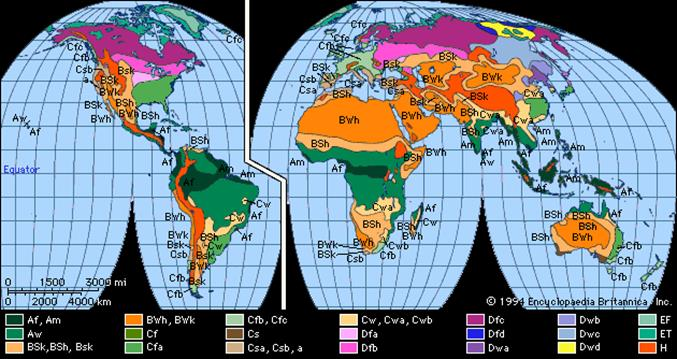
\includegraphics[width=0.9\textwidth, height=0.9\textheight, keepaspectratio=true]{media/image010.jpg}
\caption{World viewed as Köppen Climate Zones \protect \label{fig:world-viewed-as-kppen-climate-zones}}
\end{figure}

And a more basic view with monthly dry bulb temperature and dew point temperatures for these zones (Northern Hemisphere).

\begin{figure}[hbtp] % fig 15
\centering
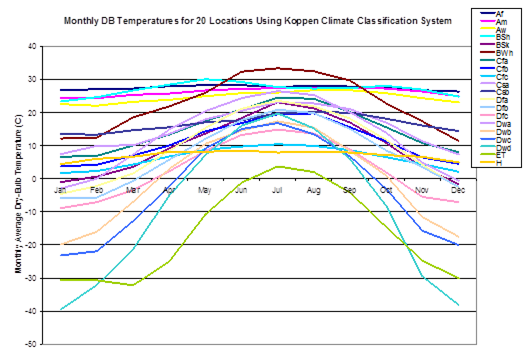
\includegraphics[width=0.9\textwidth, height=0.9\textheight, keepaspectratio=true]{media/image011.png}
\caption{Monthly Dry Bulb Temperatures in Köppen Climates (Northern Hemisphere) \protect \label{fig:monthly-dry-bulb-temperatures-in-kppen}}
\end{figure}

\begin{figure}[hbtp] % fig 16
\centering
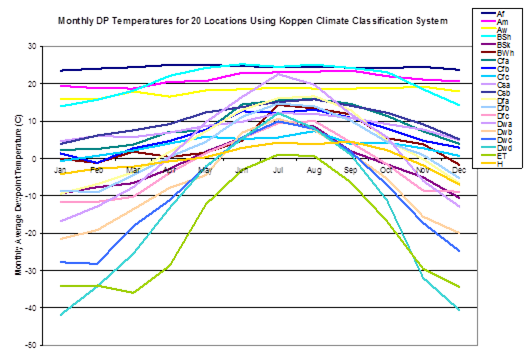
\includegraphics[width=0.9\textwidth, height=0.9\textheight, keepaspectratio=true]{media/image012.png}
\caption{Monthly Dew Point in Köppen Climates (Northern Hemisphere) \protect \label{fig:monthly-dew-point-in-kppen-climates-northern}}
\end{figure}
